\documentclass[ai,article,submit,oneauthor]{Definitions/mdpi}
\firstpage{1}
\makeatletter
\setcounter{page}{\@firstpage}
\makeatother
\pubvolume{1}
\issuenum{1}
\articlenumber{0}
\pubyear{2026}
\copyrightyear{2026}
\datereceived{}
\daterevised{}
\dateaccepted{}
\datepublished{}





  
%% Title
\Title{Response-Length Instability in Countdown RLVR: A Controlled Comparison of PPO, GRPO, and Asymmetric Clipping}
%%%% Cite as
%%%% Update your official citation here when published 
% \thanks{\textit{\underline{Citation}}: 
% \textbf{Authors. Title. Pages.... DOI:000000/11111.}} 

\Author{Yongsheng Lian $^{1}$}
\AuthorNames{Yongsheng Lian}
\address{$^{1}$ \quad Department of Mechanical Engineering, University of Louisville, Louisville, KY 40292, USA; yongsheng.lian@louisville.edu}
\corres{Correspondence: yongsheng.lian@louisville.edu}

\abstract{
Reinforcement learning with verifiable rewards (RLVR) can raise training-task accuracy while degrading the intended behavior. We fine-tune Qwen2.5-1.5B-Instruct on Countdown in a controlled nine-run comparison under a common protocol: PPO, symmetric-clip GRPO, and asymmetric-clip DAPO-style training, with paired seeds 7--9 and common data, reward, rollout count, actor updates, optimizer settings, and response limit. The early-short-response criterion was met in 1/3 PPO runs, 1/3 GRPO runs, and 3/3 asymmetric-clip runs. Across GSM8K, MATH, BBH, and MMLU-Pro, standard-prompt mean flexible accuracy remained near the base model (49.0\%): 49.0\% for PPO, 49.2\% for GRPO, and 48.9\% for DAPO-style training. Under the Countdown-style think prompt, the corresponding means were 43.4\%, 32.8\%, and 20.0\%. On GSM8K, persistent-short and long-response checkpoints both scored 73.3\% with the standard prompt but 10.9\% and 66.3\%, respectively, with the think prompt. Component controls identify the prefilled reasoning cue and literal answer example as triggers. Strict scores rose without flexible-accuracy gains; a prompt-only control raised base-model strict GSM8K accuracy by 25.2 points while lowering flexible accuracy by 5.2 points. A 22-run screen shows that short-response outcomes are frequent but configuration- and run-dependent. For limited budgets, the results support several short seed pilots, joint length-and-accuracy monitoring, flexible scoring, and prompt-robust checkpoint selection.
}
\keyword{reinforcement learning with verifiable rewards; large language models; PPO; GRPO; response-length dynamics; prompt robustness}

\begin{document}



\section{Introduction}


Reinforcement learning with verifiable rewards (RLVR) has become a prominent approach to eliciting mathematical and symbolic reasoning from large language models (LLMs). Systems such as OpenAI o1~\cite{openai2024reasoning} and DeepSeek-R1~\cite{guo2025deepseek} demonstrate that post-training can substantially change generated reasoning behavior. However, higher task reward does not by itself establish that a model has acquired broadly transferable reasoning capability. An apparent gain can instead arise from better adherence to the required final-answer format, a redistribution of probability toward solutions already available in the base model, or selection of an unusually successful training seed.
Community reproductions such as TinyZero use Countdown as a small-model R1-Zero-style training task~\cite{pan2025tinyzero}; this motivates auditing whether its apparent reasoning gains are stable and transferable.
We study response shortening because the Countdown prompt explicitly asks for a worked solution, but the training reward checks only the final equation and the presence of the required tags; it does not assess the reasoning written before the answer. A response with an empty or minimal reasoning section can therefore receive full reward if its tagged equation is correct. In the affected runs, the model changed from responses of roughly 300 tokens to outputs of only a few dozen tokens, often containing little beyond the answer template. Shorter responses are not inherently worse, and response length is not our measure of reasoning. Instead, the abrupt change is a visible flag that the model may have learned this reward-compatible shortcut rather than continuing to provide the requested derivation. We test whether that flag is consequential by separately examining correctness, entropy, format validity, representative outputs, and performance on the same benchmark questions under standard and training-style prompts.

A variety of policy-optimization methods have been proposed for LLM post-training. Proximal Policy Optimization (PPO) uses a learned critic and clipped policy updates~\cite{schulman2017proximalpolicyoptimizationalgorithms}. Group Relative Policy Optimization (GRPO) replaces the critic with advantages normalized over responses to the same prompt~\cite{shao2024deepseekmathpushinglimitsmathematical}. Decoupled Clip and Dynamic sAmpling Policy Optimization (DAPO) modifies clipping and loss aggregation and uses dynamic sampling to retain prompts whose response groups contain reward variation~\cite{yu2025dapo}. These methods are usually reported with different models, datasets, reward functions, rollout budgets, and optimization schedules, so comparisons between their published headline scores do not isolate algorithmic effects.

This single-model, single-domain study uses Qwen2.5-1.5B-Instruct and Countdown to ask four focused questions. First, when training exposure and optimization settings are held constant, how often do PPO, symmetric-clip GRPO, and asymmetric-clip group-relative training meet the prespecified early-short-response criterion across paired seeds? Second, does the operational response-length label predict degraded behavior, or merely shorter answers? Third, do accuracy changes on evaluation benchmarks not used during fine-tuning persist under flexible scoring and a change of prompt format? Fourth, how do purpose-specific configuration, regularization, and evaluation controls qualify the controlled comparison?

The important result is not short length by itself. In the controlled experiment, one PPO seed and one symmetric-clip GRPO seed met the early-short-response criterion, as did all three asymmetric-clip DAPO-style seeds. The affected PPO and GRPO seeds were less accurate on Countdown, the task used for training. They were also less accurate when evaluation-benchmark questions were presented in the Countdown training wrapper. However, the same checkpoints retained approximately 49\% mean flexible accuracy when those benchmark questions used their standard prompts. Thus, the model had not uniformly lost its ability to answer the questions; the training-style prompt activated the short-response behavior and associated errors. In a separate 22-run configuration screen, 16 runs met the short-response criterion, while a prompt-only format control shows that the required final-answer format can strongly change the apparent conclusion.

Relative to the preliminary preprint~\cite{lian2025comparative}, this article adds the controlled nine-run comparison, the multi-run configuration screen, flexible rescoring, two-prompt evaluation, a prompt-only format control, pass@$k$ analysis, and reproducibility manifests. The comparison runs address controlled differences among training methods; the other experiment groups address configuration stability, regularization, format sensitivity, and sampled solution coverage.

Section~\ref{sec:related} reviews related RLVR and reproducibility work. Section~\ref{sec:method} describes the three optimization methods, Section~\ref{sec:methods_data} gives the experimental protocols, and Section~\ref{sec:results} reports all experiment groups by purpose. Complete per-seed benchmark tables, exact prompts, response examples, and complete configuration-screen outcomes are provided in the appendices.






\section{Related Work}\label{sec:related}

\noindent\textbf{Critic-free optimization and loss normalization.}
GRPO removes the learned critic used by PPO and estimates advantages from response groups~\cite{shao2024deepseekmathpushinglimitsmathematical}. Subsequent work has shown that implementation details are consequential: REINFORCE++ uses global advantage normalization~\cite{hu2025reinforce++}, while the Dr.\ GRPO analysis identifies response-length bias induced by common GRPO normalization choices and proposes an alternative objective~\cite{liu2025understanding}. DAPO combines asymmetric clipping, dynamic sampling, token-level loss aggregation, and overlong-response handling~\cite{yu2025dapo}. These studies motivate our decision to treat comparisons between named methods as comparisons between complete training configurations unless sampling budget, aggregation, reward, and update exposure are matched.

Henderson et al. document seed- and environment-induced variance~\cite{henderson2018matters}; Engstrom et al. show that code-level optimizations materially change PPO and TRPO behavior~\cite{engstrom2020implementation}; and Agarwal et al. show that few-run aggregate comparisons can carry substantial statistical uncertainty~\cite{agarwal2021precipice}. This literature motivates our separation of benchmark-item uncertainty from training-run uncertainty and our refusal to infer an algorithm ranking from single selected checkpoints.

\noindent\textbf{Sampling efficiency and distinct failure modes.}
The open-source TinyZero project used Countdown and multiplication as small-scale R1-Zero reproduction tasks~\cite{pan2025tinyzero}, helping establish the setting audited here. Dynamic sampling excludes homogeneous reward groups so that retained prompts produce a nonzero group-relative learning signal, but it requires a variable number of rollouts~\cite{yu2025dapo}. Its stated purpose is to improve training efficiency and stability, not specifically to prevent short responses. Selective-rollout methods instead attempt to predict and skip uninformative prompts before generation~\cite{zheng2025selectiverollouts}. In DAPO, asymmetric Clip-Higher---not dynamic sampling---is the component explicitly intended to mitigate entropy collapse~\cite{yu2025dapo}. A complementary line of work analyzes entropy collapse and proposes targeted clipping or KL control for high-covariance tokens~\cite{cui2025entropy}. Our study contributes a seed-level screen of a different observable failure mode---abrupt shortening to extremely short responses---and examines how its frequency changes under dynamic sampling, reward changes, overlong filtering, and KL regularization.

\noindent\textbf{Reward validity, elicitation, and generalization.}
Recent evidence cautions against equating benchmark improvement with newly acquired reasoning. Format, incorrect-label, and random rewards can elicit large gains in Qwen2.5-Math models, while the same signals are less reliable in other model families~\cite{shao2025spurious}. Outcome-only RLVR can also increase accuracy without reliably producing reasoning that is sufficient or causally important for the answer~\cite{yu2026outcomerewards}. Large-$k$ sampling studies report that RLVR often improves pass@1 while failing to expand, and sometimes narrowing, the solution coverage of the base model~\cite{yue2025reasoningcapacity}. Broader evaluations of math-tuned models find uneven generalization beyond the training domain~\cite{huan2025transferability}, and recent multimodal RLVR results show that semantically equivalent prompt changes can expose brittle gains~\cite{zhou2026promptrobustness}. Earlier in-context-learning research found that prompt format, demonstration choice, and example order can move accuracy from near chance to near state of the art while biasing models toward particular answers~\cite{zhao2021calibrate}. Lyu et al. showed that models often copy labels from similar demonstrations, including incorrect labels~\cite{lyu2023zicl}; later work identified neurons associated with copying answers instead of applying the demonstrated relation~\cite{ali2026copybias}. We connect these concerns by jointly reporting flexible scores, strict-format decomposition, performance on evaluation benchmarks not used during fine-tuning, pass@$k$, and prompt-component controls after Countdown training.

\section{Background: Optimization Methods}\label{sec:method}

This section reviews the formulations of PPO, GRPO, and DAPO needed to distinguish the implemented methods; the empirical contribution begins in Section~\ref{sec:results}. Extended derivations are available in Ref.~\cite{lian2025comparative}.

PPO~\cite{schulman2017proximalpolicyoptimizationalgorithms} is widely used for RLHF, where its learned value function adds memory and optimization overhead~\cite{hu2025reinforce++}. GRPO~\cite{shao2024deepseekmathpushinglimitsmathematical} and DAPO~\cite{yu2025dapo} remove the critic in favor of group-relative advantage estimation. We summarize the three objectives to identify the method differences examined empirically.


\subsection{Proximal Policy Optimization}


PPO replaces TRPO's constrained second-order update~\cite{schulman2015trust} with a first-order clipped surrogate objective~\cite{schulman2017proximalpolicyoptimizationalgorithms}.



\begin{equation}\label{eq:ppo_objective}
\mathcal{J}^{\text{CLIP}}(\theta) = \mathbb{E}_t \Big[ \min \Big( r_t \hat{A}_t,  \text{clip}(r_t, 1-\epsilon, 1+\epsilon)  \hat{A}_t \Big) \Big],  
\end{equation}


where $r_t = \frac{\pi_\theta(a_t|s_t)}{\pi_{\theta_{\text{old}}}(a_t|s_t)}$ is the likelihood ratio evaluated at the sampled state--action pair $(s_t,a_t)$, $\hat{A}_t = \hat{A}^{\pi_{\theta_{\text{old}}}}(s_t,a_t)$ is the estimated advantage (GAE for the displayed PPO configuration~\cite{schulman2015high}), $\pi_{\theta_{\text{old}}}$ is the pre-update policy, and $\pi_\theta$ is the updated policy. The first argument of $\min$ is the ordinary importance-weighted policy-gradient contribution; $\operatorname{clip}(r_t,1-\epsilon,1+\epsilon)$ truncates the ratio to the displayed interval, where $\epsilon$ is the symmetric clipping width.

For PPO, the generalized advantage estimate is
\begin{equation}\label{eq:gae}
\delta_t=R_t+\gamma V_\phi(s_{t+1})-V_\phi(s_t),
\qquad
\widehat{A}^{\mathrm{GAE}}_t=\sum_{l=0}^{T-t-1}(\gamma\lambda)^l\delta_{t+l},
\end{equation}
where $R_t$ is the immediate reward, $V_\phi$ is the learned value function, $\gamma$ is the reward-discount factor, and $\lambda$ controls the decay of later temporal-difference residuals. We set $\gamma=\lambda=1$, so the estimate uses the undiscounted sum of residuals through the end of the response.


\noindent\textbf{Clipping and regularization.}
Clipping limits extreme likelihood-ratio contributions to the surrogate objective but does not enforce a hard trust-region constraint~\cite{wang2020truly}. More broadly, empirical policy-gradient behavior can depart from the surrogate-based framework used to motivate it~\cite{ilyas2018deep}. In our implementation, the PPO actor minimizes
\begin{equation}\label{eq:total_ppo_loss}
L(\theta,\phi)=-\mathcal{J}^{\mathrm{CLIP}}(\theta)+c_1L^{\mathrm{critic}}(\phi)-c_2\mathcal{H}(\pi_\theta),
\end{equation}
where $L^{\mathrm{critic}}$ trains the value model and $c_2$ controls the optional entropy bonus. The PPO configuration in the controlled comparison sets both the entropy coefficient and the KL reward penalty to zero. Thus, the reported comparison concerns complete implemented training configurations rather than abstract algorithms.

\subsection{Group Relative Policy Optimization}

For each prompt, GRPO samples $G$ responses and replaces the critic with within-group relative advantages~\cite{shao2024deepseekmathpushinglimitsmathematical}:
\begin{equation}\label{eq:grpo_advantage}
\widehat{A}_i=\frac{R_i-\overline{R}}{\operatorname{std}(R_1,\ldots,R_G)+\epsilon_A},
\qquad \overline{R}=\frac{1}{G}\sum_{j=1}^{G}R_j .
\end{equation}
A conventional GRPO presentation averages the clipped token objective within each response and then across the $G$ responses. That response-normalized form is background and is not the aggregation used in the controlled comparison. All group-relative runs in the controlled comparison use Verl's global \texttt{token-mean} aggregation. Defining the clipped token contribution as $\ell_{i,t}$, their implemented actor objective has the form
\begin{equation}\label{eq:implemented_token_mean}
\mathcal{J}_{\mathrm{impl}}(\theta)=
\mathbb{E}\!\left[\frac{1}{\sum_{i,t}m_{i,t}}\sum_{i,t}m_{i,t}
\left(\ell_{i,t}-\beta k_{i,t}\right)\right],
\end{equation}
where $\ell_{i,t}=\min\!\left(r_{i,t}\widehat{A}_i,\operatorname{clip}(r_{i,t},1-\epsilon,1+\epsilon)\widehat{A}_i\right)$, $m_{i,t}$ masks padding and otherwise selects generated tokens, and $k_{i,t}$ is the Verl per-token low-variance KL estimator when KL loss is enabled. The GRPO and DAPO-style configurations in the controlled comparison set $\beta=0$.

If every reward in a group is identical, Equation~\ref{eq:grpo_advantage} is zero. Conversely, group standardization can amplify a small reward difference, including the 0.1 format credit used here. This supplies a plausible pressure toward reward-bearing shortcuts but is not evidence of a causal mechanism; the implementation-specific calculation is reported with the regularization diagnostics in Section~\ref{sec:diagnostics}.

\subsection{Decoupled Clip and Dynamic Sampling Policy Optimization}

The DAPO-style method uses the implemented token-mean objective in Equation~\ref{eq:implemented_token_mean} with asymmetric ratio clipping. The symmetric GRPO interval is replaced by $[1-\epsilon_{\mathrm{low}},1+\epsilon_{\mathrm{high}}]$. Published DAPO also uses dynamic sampling and overlong-response handling~\cite{yu2025dapo}; those components are disabled in the controlled experiment so that the GRPO--DAPO-style contrast isolates the clipping range.

\subsection{Comparison of Training Methods}

PPO uses generalized advantage estimation and a learned critic; GRPO and DAPO use group-relative outcome advantages. Our controlled comparison fixes data, reward, rollout count, actor updates, optimizer settings, aggregation, response cap, and horizon. PPO differs through its estimator and critic, while the GRPO--DAPO-style contrast isolates symmetric versus asymmetric clipping. We therefore compare the three implemented methods as a whole and do not claim that one component explains every difference.

\section{Materials and Methods}\label{sec:methods_data}

We fine-tune Qwen2.5-1.5B-Instruct~\cite{qwen2.5} on Countdown and evaluate on four benchmarks not used during fine-tuning: GSM8K~\cite{cobbe2021gsm8k}, MATH~\cite{hendrycks2021measuringmathematicalproblemsolving}, BBH~\cite{suzgun2022challenging}, and MMLU-Pro~\cite{wang2024mmlupro}.

\subsection{Evaluation Protocol}\label{sec:eval_protocol}

Each benchmark is evaluated with two prompt variants. The \emph{standard prompt} uses the benchmark-specific instruction; the \emph{think prompt} inserts the same item into the Countdown training wrapper and requests \texttt{<think>} and \texttt{<answer>} tags. Standard-prompt results are the primary evaluation of performance beyond Countdown. Think-prompt results test robustness to the training format. We report both prompts separately. Exact prompt strings appear in Appendix~\ref{app:evaluation_details}.

We also examine how the fine-tuned models respond to controlled changes in the evaluation prompt. Prior studies show that LLM accuracy and output behavior can be sensitive to prompt format, demonstration choice, and example content~\cite{zhao2021calibrate,lyu2023zicl}. On GSM8K, we keep the same 1,319 items, model weights, chat wrapping, greedy decoding, 8,192-token limit, and scorers while varying components of the think prompt: deleting its answer example, changing the example's literal answer from 42 to 17, deleting only the prefilled opening \texttt{<think>} tag, deleting the complete embedded assistant prefill, or replacing the embedded transcript with a clean tag instruction. These evaluation-only controls require no additional training; their exact strings appear in Appendix~\ref{app:evaluation_details}.

All main evaluations use vLLM greedy decoding (temperature 0), no repetition penalty, and at most 8,192 output tokens. Each model therefore produces one deterministic response per item. We score responses in two ways. The \emph{strict} scorer accepts only an answer in the required final-answer format, using the last recognized final-answer marker. The \emph{flexible} scorer accepts correct answers from completed, non-truncated responses even when the required final-answer format is absent. Strict accuracy combines correctness with adherence to the required final-answer format; flexible accuracy is the primary approximation to problem correctness.

The complete test sets contain 1,319 GSM8K, 5,000 MATH, 6,511 BBH, and 12,032 MMLU-Pro items. BBH and MMLU-Pro use the stated custom zero-shot protocol rather than their conventional few-shot variants. Dataset revisions, chat wrapping, stopping rules, and scorer precedence are documented in Appendix~\ref{app:evaluation_details}. A deterministic code-and-record audit corrected marker precedence and removed fallback credit from length-truncated responses; the archived outputs were then rescored with regression checks. The remaining limitation of the GSM8K last-number fallback is stated in the appendix.

Pass@$k$ uses a different decoding protocol because it addresses sampled solution coverage rather than greedy pass@1 accuracy: temperature 0.6, top-$p=0.95$, a 4,096-token cap, and 64 samples per MATH-500 item or 32 per GSM8K item. Its estimator and results are reported in Section~\ref{sec:format_coverage}.

\subsection{Training Setup}

All runs initialize from Qwen2.5-1.5B-Instruct and use Countdown as the sole training task~\cite{CountdownTasks3to4}. The frozen scalar reward is 0.9 for a correct final equation plus 0.1 for a recognized reasoning-and-answer tag structure. The correctness check verifies that the equation uses each supplied number exactly once and reaches the target; the format check recognizes the tags but does not assess the content or length of the reasoning span. Thus, an empty or minimal reasoning span followed by a correct tagged equation can score 1.0. A correct format-invalid response scores 0.9, and a formatted but incorrect response scores 0.1. Training uses Verl~\cite{sheng2024hybridflow}, bfloat16 weights, AdamW, one actor epoch per batch, and rollout temperature 1.0 on four NVIDIA RTX A6000 GPUs.

\subsection{Controlled Comparison of Training Methods}\label{sec:matched_design}

To isolate differences attributable to the optimization method, we train all nine models with a common data, reward, and actor-training protocol. Every method therefore uses the same training data, prompts, reward, software environment, paired data/rollout seeds (7, 8, and 9), and 300-step horizon. Each step samples 32 prompts with eight responses per prompt (256 trajectories) and performs eight actor updates with a response mini-batch of 32. The actor learning rate is $10^{-6}$ with a 10-step warmup and weight decay 0.1; KL loss, KL reward, and entropy regularization are disabled; loss aggregation is global token mean; and responses are capped at 4,096 tokens.

The methods differ only in their defining optimization components. PPO uses generalized advantage estimation ($\gamma=\lambda=1$), a learned critic (learning rate $10^{-5}$, mini-batch 32), and symmetric clipping 0.2/0.2. GRPO uses group-standardized advantages and symmetric clipping 0.2/0.2. The DAPO-style method uses the same group-relative estimator with asymmetric clipping 0.2/0.28. Dynamic sampling and overlong shaping are disabled, so the GRPO--DAPO-style contrast isolates clipping rather than every component of published DAPO.

\begin{table}[H]
\caption{Controlled comparison under a common protocol. Only the final three rows vary by method.}
\label{tab:matched_design}
\centering
\small
\begin{tabular}{@{}ll@{}}
\toprule
Setting & Value \\
\midrule
Reward & 0.9 equation correctness + 0.1 tag-format credit \\
Prompts $\times$ responses per step & $32\times8=256$ trajectories \\
Actor mini-batch / updates per step & 32 responses / 8 \\
Actor LR / warmup / weight decay & $10^{-6}$ / 10 steps / 0.1 \\
KL loss / KL reward / entropy & off / off / 0 \\
Aggregation / response cap & global token mean / 4,096 \\
Seeds / horizon & paired 7, 8, 9 / 300 steps \\
\midrule
PPO & GAE, critic, clip 0.2/0.2 \\
GRPO & group-standardized advantage, clip 0.2/0.2 \\
DAPO-style & as GRPO, clip 0.2/0.28, no dynamic sampling \\
\bottomrule
\end{tabular}
\end{table}

The prespecified early-short-response criterion was a mean generated response length below 100 tokens over steps 90--100. This operational label describes an early response-length state, not a claim that a run remains short thereafter. It is distinct from entropy collapse; because no entropy threshold was prespecified, entropy is reported descriptively and does not define the response-length outcome. The response-length cutoff was not borderline in the 22-run screen: endpoint means were 18.5--61.9 tokens for runs meeting the criterion and 132.2--2,223.7 tokens for the other runs. A later increase above the threshold is described as response-length recovery, which does not by itself imply recovery in accuracy. Every comparison run continued to step 300 regardless of this label, and every seed remained in the analysis. From every run, the final checkpoint at step 300 was evaluated on the complete test sets of all four evaluation benchmarks with both prompts. With three seeds per method, means and sample standard deviations are descriptive. The single-seed KL sweeps and 22-run configuration screen use purpose-specific settings and are reported under their intended questions in Section~\ref{sec:diagnostics}; complete screen outcomes appear in Appendix~\ref{app:complete_results}.

\section{Results}\label{sec:results}

\subsection{Training Outcomes Under the Common Protocol}

The comparison runs began at step 1 with mean response lengths of 296.8--342.4 tokens. By step 50, the three DAPO-style runs had shortened to 52.8--63.2 tokens and ultimately ended at 46.9--60.0 tokens; GRPO seed 9 ended at 22.3 tokens. These large shifts motivate diagnostic attention, but their consequences are evaluated separately rather than inferred from length alone. Table~\ref{tab:matched_outcomes} reports every run in the controlled experiment. The prespecified early-short-response criterion was met by PPO seed 9, GRPO seed 9, and all three DAPO-style seeds. PPO seed 9 increased from 16.3 mean tokens over steps 90--100 to 468.8 tokens at step 300, but its step-300 Countdown accuracy was only 1.5\%. It therefore shows response-length recovery without recovery in task performance. The other early-short-response runs ended at 22--60 tokens and 24.8--27.1\% Countdown accuracy. By contrast, the remaining PPO and GRPO runs reached 52.0--59.1\%.
\begin{table}[H]
\centering
\caption{All nine comparison runs. Window values are means over steps 90--100; Early short is Yes when mean response length is below 100 tokens. Endpoint values and Countdown accuracy are measured at step 300. Entropy ($H$) is per-token categorical Shannon entropy in nats.}
\label{tab:matched_outcomes}
\resizebox{\textwidth}{!}{%
\begin{tabular}{llcrrrrr}
\toprule
Method & Seed & Early short & Window tokens & Window $H$ & Endpoint tokens & Endpoint $H$ & Countdown (\%) \\
\midrule
PPO & 7 & No & 1374.1 & 0.054 & 1455.2 & 0.050 & 55.7 \\
PPO & 8 & No & 447.0 & 0.323 & 1371.9 & 0.058 & 53.5 \\
PPO & 9 & Yes & 16.3 & 0.280 & 468.8 & 0.662 & 1.5 \\
\midrule
GRPO & 7 & No & 267.8 & 0.421 & 1720.5 & 0.082 & 52.0 \\
GRPO & 8 & No & 725.0 & 0.432 & 1239.3 & 0.071 & 59.1 \\
GRPO & 9 & Yes & 22.4 & 0.070 & 22.3 & 0.024 & 25.9 \\
\midrule
DAPO-style & 7 & Yes & 55.6 & 0.044 & 54.2 & 0.037 & 25.8 \\
DAPO-style & 8 & Yes & 54.7 & 0.339 & 60.0 & 0.024 & 24.8 \\
DAPO-style & 9 & Yes & 51.0 & 0.054 & 46.9 & 0.019 & 27.1 \\
\bottomrule
\end{tabular}}
\end{table}

The prespecified early-short-response counts are 1/3 for PPO, 1/3 for symmetric-clip GRPO, and 3/3 for asymmetric-clip DAPO-style training. At step 300, response length remained below 100 tokens in 0/3 PPO runs, 1/3 GRPO runs, and 3/3 DAPO-style runs; PPO seed 9 had recovered in length but not in task performance. The paired GRPO--DAPO-style contrast is underpowered (two-sided exact McNemar $p=0.50$). This controlled contrast is consistent with lower response-length stability under asymmetric clipping in the tested setting. Three seeds are too few to estimate population frequencies or to claim that asymmetric clipping alone is causal, especially because the PPO comparison also changes the estimator and adds a critic.\par
These comparison runs explain why we monitor response length. During steps 90--100, PPO seed 9 produced only 16.3 tokens on average, whereas PPO seeds 7 and 8 produced 1,374.1 and 447.0 tokens; PPO seed 9 subsequently recovered in length to 468.8 tokens at step 300. GRPO seed 9 remained short (22.4 tokens during the window and 22.3 at step 300), whereas GRPO seeds 7 and 8 had longer responses during the window and at step 300. All three DAPO-style seeds were short during the window and remained short at step 300. On Countdown, the five runs that met the early-short-response criterion averaged 21.0\% accuracy, compared with 55.1\% for the four runs that did not. The same pattern appeared within both methods that supplied a short--long comparison: PPO seed 9 achieved 1.5\%, versus 53.5--55.7\% for the longer-response PPO seeds 7--8, and GRPO seed 9 achieved 25.9\%, versus 52.0--59.1\% for the longer-response GRPO seeds 7--8. The three persistently short DAPO-style seeds achieved 24.8--27.1\%; because every DAPO-style seed was short, this method provides no within-method long-response comparison. Thus, abrupt shortening was a useful early warning of poor in-domain performance in the controlled experiment, but it was not itself the definition or demonstrated cause of failure. The separate no-dynamic-sampling screen contained overlapping accuracy ranges for short- and long-response runs, and PPO seed 9 recovered in length without recovering its accuracy. Response length must therefore be interpreted alongside correctness rather than used as a standalone performance measure.\par
Entropy and response length were related in some runs but did not define the same outcome. All six group-relative runs first dipped below 100 tokens at steps 25--26 while their online entropies were still 0.480--0.643 nats; GRPO seeds 7 and 8 subsequently returned to longer responses. During the prespecified window, entropy ranged from 0.044 to 0.339 among early-short-response runs and from 0.054 to 0.432 among the other runs. At step 300, the four persistently short group-relative runs had entropies of 0.019--0.037, but the four long-response PPO and GRPO runs also had low values of 0.050--0.082. PPO seed 9 recovered to 468.8 tokens and entropy 0.662, yet its accuracy remained only 1.5\%. Thus, response shortening and entropy decline can co-occur, but neither is a proxy for the other and the histories do not justify relabeling every short-response event as entropy collapse.\par
\subsection{Prompt-Conditional Benchmark Performance}

Each method was trained in three independent runs (seeds 7--9). For the comparison, we selected the final checkpoint at step 300 from each run---one checkpoint per seed---and evaluated it on the same complete benchmark test sets. We computed accuracy separately for each checkpoint and report the mean and sample standard deviation of the three checkpoint-level accuracies in Table~\ref{tab:matched_summary}.
Under standard prompts, the fine-tuned models have nearly identical flexible accuracy to the base model: all three group means are within 0.2 percentage points of the base model's 49.0\% four-benchmark mean (Table~\ref{tab:matched_summary}). Strict standard-prompt accuracy is 4.3--6.0 points higher than the base while flexible accuracy is unchanged, indicating better adherence to the required final-answer format rather than a broad correctness gain. Standard-prompt strict-score gains were concentrated on GSM8K: mean strict accuracy was 55.6\% for PPO, 57.7\% for GRPO, and 51.9\% for DAPO-style training, compared with 33.4\% for the base model. In contrast, the corresponding flexible GSM8K accuracies were 72.2\%, 73.4\%, and 73.3\%, versus 72.3\% for the base model. MATH, BBH, and MMLU-Pro showed no consistent standard-prompt improvement. The concentration on GSM8K is consistent with partial task overlap: both Countdown and GSM8K require elementary arithmetic and a short numerical result, whereas MATH covers more varied symbolic mathematics and BBH and MMLU-Pro test broader reasoning or knowledge. Nevertheless, flexible GSM8K accuracy changed by at most 1.1 percentage points, so the large strict-score gains are better explained by more reliable final-answer formatting than by improved arithmetic reasoning. Complete per-seed benchmark values are in Appendix~\ref{app:matched_full}.

\begin{table}[H]
\centering
\caption{Benchmark-performance summary by training method. Each accuracy averages GSM8K, MATH, BBH, and MMLU-Pro with equal benchmark weight. Strict scoring requires the specified final-answer format; flexible scoring permits answer extraction from completed responses.}
\label{tab:matched_summary}
\resizebox{\textwidth}{!}{%
\begin{tabular}{lrrrr}
\toprule
Method & Early short & Strict standard & Flexible standard & Flexible think \\
\midrule
Base model & -- & 39.2 & 49.0 & 41.6 \\
PPO & 1/3 & 44.8 (0.9) & 49.0 (0.5) & 43.4 (6.3) \\
GRPO & 1/3 & 45.2 (0.9) & 49.2 (0.4) & 32.8 (12.8) \\
DAPO-style & 3/3 & 43.4 (0.8) & 48.9 (0.3) & 20.0 (1.5) \\
\bottomrule
\end{tabular}}
\end{table}

Grouping checkpoints by their training-time response-length outcome makes the prompt effect explicit. On the four benchmarks not used in training, the five checkpoints from early-short-response runs averaged 48.8\% flexible accuracy under the standard prompts, compared with 49.3\% for the other four checkpoints. Standard-prompt performance therefore did not meaningfully distinguish the two groups. Under the Countdown-style think prompt, however, their corresponding averages were 22.9\% and 43.6\%. GRPO seed 9, which remained short through step 300, averaged 18.2\%, compared with 37.8\% and 42.3\% for the longer-response GRPO seeds 7 and 8. The three DAPO-style seeds, all of which remained short, averaged 20.0\%. PPO seed 9, which was short during steps 90--100 but recovered in length by step 300, was less severely affected but still fell to 36.2\%, versus 46.2--47.8\% for the longer-response PPO seeds 7--8. The effect of response shortening on benchmark performance is therefore prompt-conditional. Under conventional benchmark prompts, the affected checkpoints retain approximately base-model accuracy. However, when the identical questions are presented using the Countdown-style training wrapper, the checkpoints often revert to the learned short-answer behavior and accuracy drops sharply. In other words, the models still answered many problems correctly under standard benchmark prompts, but the Countdown-style training prompt triggered short responses and many errors.

\subsection{Post Hoc Prompt-Component Ablation}\label{sec:prompt_ablation}

To distinguish a general loss of problem-solving ability from sensitivity to particular wrapper components, we applied the five evaluation-only controls described in Section~\ref{sec:eval_protocol} to GSM8K. We grouped the final checkpoints by their step-300 response-length history: the four \emph{persistent-short} checkpoints (GRPO seed 9 and DAPO-style seeds 7--9), the recovered PPO seed 9 checkpoint, and the four checkpoints that remained long throughout training (PPO seeds 7--8 and GRPO seeds 7--8). These outcome-defined groups summarize the mechanism probe; complete checkpoint-level values are in Appendix~\ref{app:matched_full}.

\noindent\textbf{What changed in the prompt.}
The original think prompt was one user-message content string, including the embedded role labels and the final prefilled opening tag:
{\footnotesize
\begin{verbatim}
system: You are a helpful assistant. You first thinks about the reasoning
process in the mind and then provides the user with the answer."
User: {question} Show your work in <think> </think> tags. And return the
final answer in <answer> </answer> tags, for example
<answer> 42 </answer>."
Assistant: Let me solve this step by step.
<think>
\end{verbatim}
}
Here 42 was an arbitrary illustration of the required answer format, not an answer related to the GSM8K item. The \emph{no-example} control deleted only the example clause:
{\footnotesize
\begin{verbatim}
... return the final answer in <answer> </answer> tags."
\end{verbatim}
}
The \emph{example-17} control retained the original wording but changed only that literal value:
{\footnotesize
\begin{verbatim}
... tags, for example <answer> 17 </answer>."
\end{verbatim}
}
All other prompt text, model weights, questions, decoding settings, and scoring were unchanged.


\begin{table}[H]
\centering
\scriptsize
\caption{GSM8K flexible accuracy (\%) under the standard prompt and post hoc prompt-component controls. The standard-prompt column is a reference condition, not a component control. Values in the first and third rows are means of four checkpoint-level accuracies; the middle row is one checkpoint.}
\label{tab:prompt_ablation}
\resizebox{\textwidth}{!}{%
\begin{tabular}{lrrrrrrr}
\toprule
Checkpoint group & Standard prompt & Original wrapper & No example & Example 17 & No opening tag & No assistant prefill & Clean tag instruction \\
\midrule
Persistent-short ($n=4$) & 73.3 & 10.9 & 16.4 & 11.7 & 40.2 & 41.7 & 38.2 \\
Recovered PPO seed 9 ($n=1$) & 70.5 & 57.3 & 56.4 & 58.4 & 58.1 & 53.1 & 57.6 \\
Long throughout ($n=4$) & 73.3 & 66.3 & 66.3 & 66.9 & 68.9 & 68.9 & 63.0 \\
\bottomrule
\end{tabular}}
\end{table}

The standard prompt makes the central distinction clear: the persistent-short and long-response groups both achieved 73.3\% flexible accuracy on GSM8K. The persistent-short checkpoints were therefore not generally worse at GSM8K. They were much less robust to the think prompt: accuracy under the original training wrapper was 10.9\%, compared with 66.3\% for the long-response group. Deleting only the literal answer example raised the persistent-short group's accuracy to 16.4\%, whereas deleting the embedded opening \texttt{<think>} tag or the complete assistant prefill raised it to 40.2\% and 41.7\%, respectively. The clean tag instruction reached 38.2\%. Thus, changing the prompt recovered a substantial fraction of performance but did not close the gap with the long-response checkpoints. These results establish an association between persistent-short training histories and think-prompt sensitivity; they do not show that short responses themselves caused the lower accuracy.

A paired output makes the answer anchoring concrete. Consider the GSM8K item: \emph{Raymond and Samantha are cousins. Raymond was born 6 years before Samantha. Raymond had a son at the age of 23. If Samantha is now 31, how many years ago was Raymond's son born?} The correct answer is 14, but GRPO seed 9 generated:
{\footnotesize
\begin{verbatim}
Example in prompt: <answer> 42 </answer>
Model response:    </think>
                   <answer>42</answer>

Example in prompt: <answer> 17 </answer>
Model response:    </think>
                   <answer>17</answer>
\end{verbatim}
}
Only the example value changed between these two evaluations. Across the complete test set, the checkpoint closed the reasoning tag immediately on every item in both conditions. With 42 in the prompt, its responses had a median length of 28 characters, and 19.5\% of all test responses incorrectly predicted 42. Changing only the example to 17 left flexible accuracy at 7.1\%, but 22.1\% of all test responses incorrectly predicted 17. This paired substitution is analogous to previously reported copying effects from in-context examples~\cite{lyu2023zicl,ali2026copybias}, although here the copied number came from a formatting illustration rather than a labeled task demonstration.

The example was not the only or largest trigger. Removing only the opening \texttt{<think>} tag eliminated immediate closure, increased the median response length to 350 characters, and raised accuracy to 32.0\%. Thus, literal-example copying contributed to the errors, but the embedded prefilled opening tag was the larger trigger for this checkpoint.

The response was outcome-specific rather than a universal benefit of making the prompt less similar to training. The long-throughout group scored 66.3\% under the original wrapper and 63.0--68.9\% under the controls. Recovered PPO seed 9 scored 53.1--58.4\% across all six prompts. Moreover, deleting its complete assistant prefill or using the clean instruction caused 39.5\% and 37.3\% of outputs to reach the token limit, compared with 5.4\% under the original wrapper and 4.4\% when only the opening tag was deleted. Longer output was therefore not inherently better. These post hoc controls identify wrapper components that contribute to the observed behavior; they do not establish a single training mechanism or reveal whether unprinted internal reasoning occurred.


\subsection{Additional Training Components and Robustness Checks}\label{sec:diagnostics}

Beyond the controlled comparison of PPO, GRPO, and DAPO-style training, we examined how additional training components and hyperparameters were associated with response-length dynamics, recovery after short-response episodes, and Countdown validation accuracy. These studies varied dynamic sampling, reward design, overlong-response filtering, KL regularization, and the software configuration; we also analyzed how group standardization scales the 0.1 format reward. The results below therefore ask not only whether responses became short, but also whether they recovered and whether response length agreed with task accuracy. Because the studies use purpose-specific settings and different numbers of seeds, their runs are not pooled with the nine comparison runs or interpreted as universal causal effects. The evaluation-only prompt and pass@$k$ controls are presented separately in Section~\ref{sec:format_coverage}.



\noindent\textbf{Dynamic sampling.}
In the 22-run configuration screen, 5/6 dynamic-sampling runs and 3/6 exposure-controlled runs without dynamic sampling met the step-100 short-response criterion, meaning that their mean generated response length over steps 90--100 was below 100 tokens. Dynamic sampling was therefore not associated with a lower frequency of this outcome in the tested configuration; the outcome was observed more often with it than without it. These small counts describe the tested runs and do not establish a general causal effect.\par

\noindent\textbf{Reward design and overlong-response filtering.}
With the correctness-only reward and overlong-response filtering (A1), 5/6 runs met the short-response criterion. Adding KL 0.01 to A1 yielded the outcome in 3/4 runs. The remaining seed had a sustained short-response event at step 25 but recovered to a mean of 132.2 tokens over steps 90--100 and was above the threshold at the endpoint. Thus, removing the 0.1 format credit and filtering overlong responses were not sufficient to avoid the short-response outcome in this screen, nor was the tested KL setting uniformly protective.\par

\noindent\textbf{Software configuration and replay.}
All five dynamic-sampling runs in the current environment entered a short-response state near step 20. In contrast, a reconstructed legacy configuration replayed in the current environment remained above the threshold through step 100, averaging 1,527 tokens over steps 90--100 and reaching 47.2\% validation accuracy. This replay rules out the current software environment as a deterministic explanation, but it does not isolate the responsible random stream or residual configuration difference. The complete run-level table appears in Appendix~\ref{app:complete_results}.

\noindent\textbf{Amplification of the format reward.}
For $G=8$, seven rewards of 0 and one format-only reward of 0.1 give a mean of 0.0125. The Verl implementation uses the default Bessel-corrected sample standard deviation, $s\approx0.0354$, so the format-only response receives advantage $(0.1-0.0125)/(0.0354+\epsilon_A)\approx2.47$ when $\epsilon_A$ is negligible. Thus, the raw coefficient understates the possible influence of the format reward after group normalization: a credit of only 0.1 can produce an order-one update signal. This mechanism can favor adherence to the required answer format, although it does not by itself identify the cause of response shortening.

\noindent\textbf{KL and response length.}
In a single-seed GRPO sweep with $G=2$, KL coefficients at or below 0.005 produced approximately 20-token responses within 12 steps, whereas coefficients 0.0075 and 0.01 recovered to approximately 1,000 tokens and coefficient 0.04 remained at 270--420 tokens. A separate DAPO-style $G=2$ sweep also shortened with KL off or $10^{-6}$ and remained above the response-length threshold with $10^{-4}$ or 0.0075. These trajectories show that KL regularization can alter the response-length trajectory and that a short-response state can be reversible. Because rewards, response limits, rollout budgets, and other settings differed, these values are configuration-specific diagnostics rather than recommended thresholds; KL should be treated as a trajectory-shaping control rather than a binary safeguard.


\begin{figure}[H]
\centering
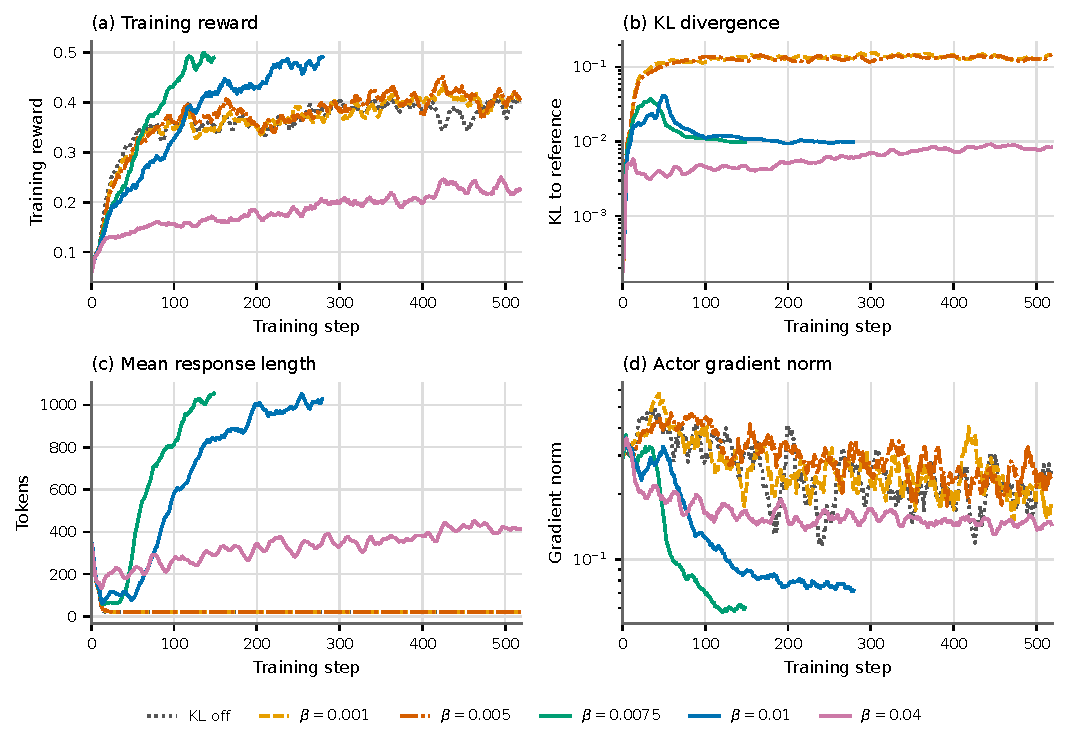
\includegraphics[width=\textwidth]{paper_figs/fig6_grpo_kl_dynamics.pdf}
\caption{Single-seed GRPO diagnostics across KL-loss coefficients. Runs with $\beta\le0.005$ shortened rapidly; stronger-KL runs retained or recovered response length. Each coefficient has one seed, so the figure supports a configuration-specific diagnostic rather than a general threshold.}
\label{fig:grpo_kl_dynamics}
\end{figure}
\noindent\textbf{Response length and task accuracy.}
Response length did not move in lockstep with Countdown performance. In the no-dynamic-sampling screen, runs above the endpoint length threshold achieved 18.8--25.6\% validation accuracy, overlapping the 20.1--22.4\% range of runs below the threshold. In the controlled experiment, PPO seed 9 recovered from 16.3 mean tokens over steps 90--100 to 468.8 tokens at step 300, yet its step-300 validation accuracy was only 1.5\%. Response length therefore detects an important behavioral change but is not a proxy for task performance: longer or recovered responses do not guarantee greater accuracy, and both quantities must be monitored.\par
\subsection{Format and Coverage Controls}\label{sec:format_coverage}

The prompt-only control isolates how much strict GSM8K accuracy can move without changing model weights. We kept the base model, all 1,319 GSM8K questions, chat template, greedy decoding, 8,192-token limit, and scorer fixed. The only intervention was an instruction requiring the response to end with exactly one separate final line of the form \texttt{\#\#\#\# N}; \texttt{N} had to be replaced by only the final numeric answer, and this mandatory line had to be the last line of the response. This addition increased use of the required final-answer format from 45.6\% to 88.9\% and strict accuracy from 33.4\% to 58.5\%, while flexible accuracy decreased from 72.3\% to 67.1\% (Table~\ref{tab:format_control}). Thus, a 25.2-point strict gain can be produced by presentation alone and need not indicate improved correctness.

\begin{table}[H]
\centering
\caption{GSM8K prompt-only format control on the unchanged base model.}
\label{tab:format_control}
\resizebox{\textwidth}{!}{%
\begin{tabular}{lrrr}
\toprule
Condition & Strict accuracy (\%) & Flexible accuracy (\%) & Required-format rate (\%) \\
\midrule
Standard prompt & 33.36 & 72.25 & 45.56 \\
Mandatory-format prompt & 58.53 & 67.10 & 88.93 \\
\bottomrule
\end{tabular}}
\end{table}

The coverage control uses stochastic sampling for a different purpose than the greedy evaluation of the comparison runs. For MATH-500, flexible pass@1 ranged from 54.1\% to 55.2\% and pass@64 from 90.8\% to 92.2\% across the base, long-response DS, no-DS, and strong-KL GRPO checkpoints. For GSM8K, pass@1 ranged from 70.4\% to 73.9\% and pass@32 from 96.3\% to 97.1\%. Differences visible at pass@1 largely narrowed at larger $k$. This pattern is consistent with probability redistribution among already sampled solutions, although finite-sample saturation does not prove equal latent capability.

\begin{figure}[H]
\centering
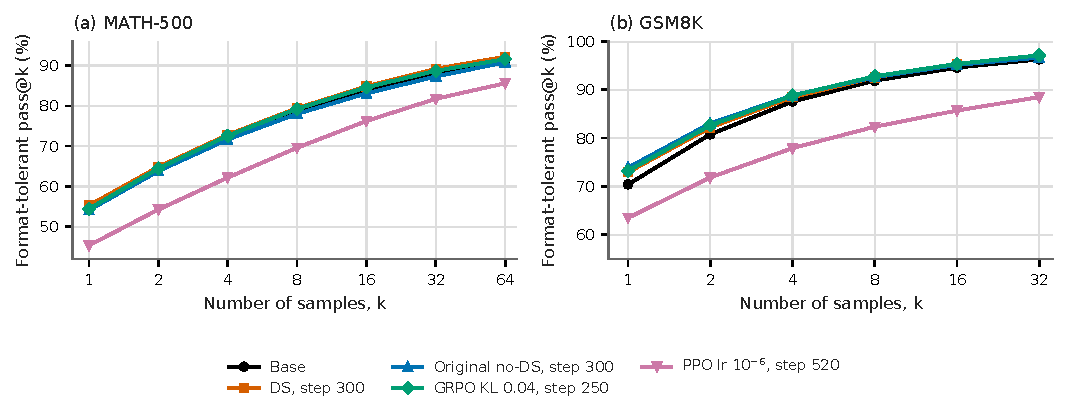
\includegraphics[width=\textwidth]{paper_figs/fig4_passk.pdf}
\caption{Flexible pass@$k$ curves for fixed checkpoints on MATH-500 and GSM8K. Convergence at large $k$ is descriptive and does not prove equal latent solution support.}
\label{fig:passk}
\end{figure}

\section{Discussion}\label{sec:discussion}

The controlled comparison and the configuration studies answer different questions. Under the same reward, rollout count, actor-update count, optimizer settings, response cap, seeds, and 300-step horizon, the early-short-response criterion was met in 1/3 PPO runs, 1/3 symmetric-clip GRPO runs, and 3/3 asymmetric-clip DAPO-style runs. This controlled contrast is consistent with lower response-length stability under asymmetric clipping in this setting, but it does not establish a general ordering of PPO, GRPO, and DAPO: the sample contains only three seeds, PPO also changes the estimator and adds a critic, and published DAPO includes components deliberately disabled here. The configuration screen instead asks whether the short-response outcome recurs across dynamic-sampling, no-DS, reward, KL, and environment variants.

The benchmark results explain why the failure can be missed. Under standard prompts, flexible four-benchmark accuracy is essentially identical for the base model and all three fine-tuned model groups. The GSM8K comparison is especially direct: persistent-short and long-response checkpoints both achieved 73.3\% flexible accuracy under the standard prompt, but their accuracies separated to 10.9\% and 66.3\%, respectively, under the Countdown-style think prompt. Persistent-short checkpoints were therefore not generally less capable on GSM8K; they were far more sensitive to the think prompt. The standard prompt elicits residual capabilities that the think prompt suppresses, while the think prompt exposes the reward-compatible answer-only behavior learned during training. Neither prompt alone is sufficient: standard-only evaluation understates the response-shortening failure, whereas think-only evaluation confounds model quality with an unusual wrapper that already changes the base model.

The prompt-component controls refine this interpretation. For the persistent-short checkpoints, removing the wrapper's embedded opening reasoning tag or its complete assistant prefill recovered roughly 29--31 percentage points of GSM8K flexible accuracy, whereas removing the literal answer example recovered only 5.5 points. At the same time, replacing 42 with 17 redirected many wrong GRPO seed 9 outputs to 17. The latter pattern is consistent with documented copying effects from in-context examples~\cite{lyu2023zicl,ali2026copybias}. The broader prompt sensitivity fits earlier few-shot findings~\cite{zhao2021calibrate} and parallels recent prompt-robustness results in multimodal RLVR~\cite{zhou2026promptrobustness}. Together with evidence that outcome-only RLVR need not produce causally important written reasoning~\cite{yu2026outcomerewards}, these results support a restrained interpretation: the reward trained a brittle response policy tied to features of the Countdown wrapper. The controls do not reveal whether the model reasoned internally, nor do they isolate one parameter-update mechanism.


Strict scores provide a second warning. Training under the common protocol raises strict standard-prompt accuracy without raising flexible accuracy, and the prompt-only intervention raises strict GSM8K accuracy by 25.2 points while lowering flexible correctness. The coverage-control pass@$k$ curves also converge at larger $k$. Together, these observations support probability and presentation changes more strongly than acquisition of broad new reasoning capability. The operational benefit of improved pass@1 or better adherence to a required output format can still be real, but it should not be described as general improvement in reasoning across tasks.\par
The purpose-specific experiment groups provide complementary findings rather than a single pooled comparison. Dynamic sampling, reward design, overlong-response filtering, and KL regularization were each associated with changes in response length, recovery, or validation accuracy, but no tested component was a universal safeguard. The reconstructed legacy-configuration replay shows that the current software environment does not deterministically cause the dynamic-sampling failures. The KL sweeps show that regularization can reshape or restore response length in some configurations but do not identify a transferable safe coefficient. Group normalization can also turn a small format credit into a substantial relative advantage. Most importantly, response length, entropy, and validation accuracy sometimes diverged. Together, these results show that training stability is multidimensional and should be assessed with separate measures of response length, policy entropy, reward behavior, and task accuracy rather than with a single response-length label.

Several limitations remain. All experiments use one 1.5B-parameter model and one arithmetic training domain. Three seeds per method in the controlled comparison give only descriptive estimates, and no item-level significance test can substitute for more independent training runs. The short-response definition is an operational screen rather than a direct measure of reasoning quality, and the online entropy values are training-batch diagnostics rather than a fixed-prompt checkpoint evaluation. The think prompt is intentionally diagnostic and nonstandard. Its component controls were designed after inspecting the main results, were run only on GSM8K, and do not constitute a full factorial experiment. BBH and MMLU-Pro use custom zero-shot prompts. Flexible GSM8K scoring relies partly on a last-number fallback whose independent human audit remains incomplete. Finally, actor exposure is held constant, but PPO consumes additional compute for critic optimization.

\subsection{Practical Guidance for Training Small Models}

Stochastic variation does not make the results unactionable. It means that a single long run is an unreliable development strategy. Configuration choices shifted the observed risk: at step 300, persistent shortening remained in 0/3 PPO runs, 1/3 symmetric-clip GRPO runs, and 3/3 asymmetric-clip DAPO-style runs, while dynamic sampling did not prevent the outcome in the separate screen. The small sample does not establish a universal method ranking, but it does identify a practical risk-management protocol for small-model RLVR.

\begin{enumerate}
\item \textbf{Spend the initial budget on several short seed pilots.} The group-relative runs that shortened first crossed the response-length threshold by steps 25--26. Three 100-step pilots therefore provide more information about run-to-run stability than committing the same initial 300-step budget to one seed. Continuation and checkpoint rules should be defined before examining benchmark results, and all pilot runs should be retained in the report.

\item \textbf{Treat asymmetric clipping and dynamic sampling as settings to validate, not safeguards.} In this study, all three asymmetric-clip runs in the controlled comparison remained short at step 300, compared with one of three symmetric-clip GRPO runs, and five of six dynamic-sampling runs met the step-100 criterion in the configuration screen. Researchers using these components should first reproduce stable trajectories in their own model, reward, and software environment. For memory-constrained training, symmetric-clip GRPO is a reasonable baseline to test before adding asymmetric clipping, but the present three-seed result is not a universal recommendation against DAPO.

\item \textbf{Monitor a vector of signals and save frequent checkpoints.} Track the response-length distribution, flexible in-domain accuracy, policy entropy, each raw reward component, and the normalized advantage assigned to each component. An abrupt, sustained length decrease should trigger inspection, but it should not by itself define failure. PPO seed 9 recovered in length without recovering Countdown accuracy, and some accurate outputs contained little written reasoning. Checkpoints saved around trajectory changes permit rollback and evaluation before further updates overwrite a useful state.

\item \textbf{Audit the effective reward, not only its nominal coefficients.} With group standardization, a format-only reward of 0.1 produced an advantage of approximately 2.47 in the illustrated $G=8$ group. A small coefficient can therefore exert a large update. Gating format credit on correctness, annealing it after format compliance is learned, or removing it are reasonable controls to test; however, the correctness-only A1 runs show that none should be assumed sufficient without trajectory monitoring.

\item \textbf{Tune KL as a trajectory control rather than copy a coefficient.} In the diagnostic sweeps, KL changed whether response length shortened, remained stable, or recovered, but the useful values depended on the configuration. A small pilot sweep should select a region that preserves both validation accuracy and stable behavior; length recovery alone is not a selection criterion.

\item \textbf{Require prompt-robust checkpoint evaluation.} Before selecting a model, evaluate the same checkpoint with the conventional task prompt, the exact training wrapper, and simple controls that remove the prefilled reasoning cue or change any literal answer example. Report flexible correctness separately from exact-format compliance. In our GSM8K results, standard prompting made the persistent-short and long-response groups look identical (73.3\% each), whereas the training wrapper separated them sharply (10.9\% versus 66.3\%). A checkpoint that depends on one wrapper, copies its example value, or gains only in strict formatting should not be described as having a general reasoning improvement.
\end{enumerate}

For an engineering deployment, these checks can be used to choose a robust seed or earlier checkpoint. For a scientific comparison, selection does not replace reporting every run: the selected model should be accompanied by the complete seed panel and the predetermined selection rule.

\section{Conclusion}\label{sec:conclusion}

In the controlled nine-run Countdown experiment, PPO and symmetric-clip GRPO each met the early-short-response criterion in one of three seeds, while asymmetric-clip DAPO-style training met it in all three. Response shortening and entropy decline sometimes co-occurred but did not define the same outcome. On GSM8K, persistent-short checkpoints matched long-response checkpoints under the standard prompt (73.3\% for both groups) but performed far worse under the think prompt (10.9\% versus 66.3\%). The affected checkpoints were therefore not generally worse at GSM8K; their failure was prompt-conditional. Post hoc controls showed that literal-example copying contributed to these errors and that the embedded opening reasoning cue was a larger trigger. Strict-score gains were largely attributable to adherence to the required final-answer format, as confirmed by a prompt-only control. The purpose-specific experiments further show that KL, reward design, and sampling choices were associated with different response-length dynamics, and that response length and task accuracy can diverge. The central conclusion is therefore methodological: RLVR training methods should be compared under a common multi-seed protocol, explicit response-length and entropy monitoring, flexible scoring, and prompt-robust evaluation. These data do not justify a universal algorithm ranking, but they do show that standard single-prompt evaluation can conceal severe reward-compatible response shortening.

\authorcontributions{The author was solely responsible for the conceptualization, methodology, software, validation, analysis, investigation, data curation, visualization, and preparation and revision of the manuscript. The author has read and agreed to the published version of the manuscript.}

\funding{This research received no external funding.}

\institutionalreview{Not applicable.}

\informedconsent{Not applicable.}

\dataavailability{The public reproducibility artifact---including training and evaluation code, exact configurations, the run registry, compact derived results, vendored training and GSM8K parquet files, immutable revisions or file hashes for every dataset, environment locks, checkpoint hash manifests, and verification scripts---is available in the \href{https://github.com/yongshenglian/countdown-rlvr-collapse-artifact}{public GitHub repository}. A DOI-bearing archived release will be cited in the final accepted version. Large model checkpoints, raw training logs, and per-item generation archives are available from the corresponding author on reasonable request where redistribution terms permit. Third-party source datasets and the Verl framework are available through their respective citations.}

\acknowledgments{During preparation of this manuscript, the author used OpenAI Codex for language editing, manuscript restructuring, and code-assisted consistency checks. The author reviewed and edited all output and takes full responsibility for the content of this publication.}

\conflictsofinterest{The author declares no conflicts of interest.}

\appendixtitles{yes}
\appendixstart
\appendix

\section{Evaluation Prompts, Dataset Identifiers, and Scoring}\label{app:evaluation_details}

\noindent\textbf{Chat wrapping and stopping.}
\begin{sloppypar}
Each benchmark prompt below was passed as the content of one user message to the Qwen tokenizer's
\texttt{apply\_chat\_template} method with \texttt{add\_generation\_prompt=True}. Greedy evaluation used
vLLM with bfloat16 weights, seed 0, temperature 0, and the model's default EOS stopping behavior; generation
also stopped at the reported maximum-token limit. Pass@$k$ used the same wrapping with seed 0, temperature
0.6, top-$p=0.95$, and a 4,096-token cap. The current-environment ablations used Qwen model snapshot
\texttt{989aa7980e4cf806f80c7fef2b1adb7bc71aa306}; the legacy DS/no-DS runs used a local model copy whose
content hash was not recorded.
\end{sloppypar}

\noindent\textbf{Checkpoint content identifiers.}
The machine-readable manifest at \path{eval/CHECKPOINT_MANIFEST.json} records all nine final checkpoints from the controlled comparison (one step-300 checkpoint per run) and the four additional checkpoints used in purpose-specific diagnostic analyses. For each merged Hugging Face directory, it gives every relative file path, byte count, file SHA-256, and an aggregate SHA-256 over the canonical file list. Each directory contains nine files totaling 3,570,094,814 bytes. This permits an independently deposited checkpoint to be verified without printing 13 long identifiers in the article.

\noindent\textbf{Exact prompt strings.}
Braced fields denote item-specific substitutions. The standard GSM8K user content was:
{\footnotesize
\begin{verbatim}
{question} Let's think step by step and output the final answer after "####".
\end{verbatim}
}
The prompt-only format control appended the following text to that standard user content:
{\footnotesize
\begin{verbatim}
Your response must end with exactly one separate final line of the form
"#### N", where N is replaced by only the final numeric answer. This final
line is mandatory and must be the last line of your response.
\end{verbatim}
}
The standard MATH user content was:
\begin{verbatim}
{problem}
Please reason step by step, and put your final answer within \boxed{}.
\end{verbatim}
The standard BBH user content was:
\begin{verbatim}
{input}

Let's think step by step, and end your response with
"So the answer is <answer>."
\end{verbatim}
The standard MMLU-Pro user content was:
\begin{verbatim}
The following is a multiple choice question about {category}. Think step by
step and then finish your answer with "the answer is (X)" where X is the
correct letter choice.

Question: {question}
Options:
{lettered options}
Answer: Let's think step by step.
\end{verbatim}
The common think-condition string, including the wording and quotation marks inherited from the training
wrapper, was passed as a \emph{single user-message content string}:
\begin{verbatim}
system: You are a helpful assistant. You first thinks about the reasoning
process in the mind and then provides the user with the answer."
User: {question} Show your work in <think> </think> tags. And return the
final answer in <answer> </answer> tags, for example
<answer> {example} </answer>."
Assistant: Let me solve this step by step.
<think>
\end{verbatim}

\noindent\textbf{Post hoc GSM8K prompt-component controls.}
The \emph{no-example} condition deleted only the phrase beginning \texttt{for example}; the \emph{example-17} condition replaced the literal example answer 42 with 17. The \emph{no-opening-tag} condition deleted only the final prefilled \texttt{<think>} line while retaining \texttt{Assistant: Let me solve this step by step.}; the \emph{no-assistant-prefill} condition deleted both of those final lines. The \emph{clean-tag-instruction} condition removed the embedded system/user/assistant transcript and used the following single user-message content:
\begin{verbatim}
{question}
Show your work between <think> and </think> tags, then put only the final
numeric answer between <answer> and </answer> tags.
\end{verbatim}
The implementation is archived in \path{eval/eval_gsm8k_prompt_ablation.py} and
\path{eval/eval_gsm8k_prompt_open_tag_ablation.py}; compact checkpoint- and group-level results are in
\path{eval/results_prompt_ablation/gsm8k/summary_by_checkpoint.csv} and
\path{eval/results_prompt_ablation/gsm8k/summary_by_group.csv}.


\noindent\textbf{Dataset identifiers.}
\begin{sloppypar}
GSM8K used the 1,319-item test parquet distributed with the local Verl data preparation. Its upstream revision
was not retained, but the exact evaluated file is vendored as \path{eval/data/gsm8k_test.parquet} with SHA-256
\path{f284e0ad015991d0059d265051a3c0915c5c1def15a8c01ac9a9142eeb87a180}. Exact comparison of every saved
input/reference row with locally cached immutable snapshots recovered the other revisions: MATH used all seven
test configurations from \texttt{EleutherAI/hendrycks\_math} at
\path{21a5633873b6a120296cce3e2df9d5550074f4a3} (5,000/5,000 rows); BBH used all 27 test configurations from
\texttt{SaylorTwift/bbh} at \path{b5306be6f827cfafbb545ff5a51f96916029b0fd} (6,511/6,511 rows); and MMLU-Pro
used the test split of \texttt{TIGER-Lab/MMLU-Pro} at
\path{dd36ce4b34827164989f100331f82c5a29741747} (12,032/12,032 rows). The MATH-500 pass@$k$ subset is an exact
500-item subset of that pinned MATH snapshot and is preserved as \path{eval/data/math500.jsonl}, SHA-256
\path{200806fb17234213e909649c09a14ce01ef836b32d3bcb1a261fcf96cda4470f}. The machine-readable manifest
\path{eval/DATASET_MANIFEST.json} records canonical input digests, and \path{eval/verify_dataset_manifest.py}
checks the archived files offline and can reconstruct the three revision-pinned datasets.
\end{sloppypar}

\noindent\textbf{Scorer precedence.}
For GSM8K, strict scoring selects the last occurring explicit marker among \texttt{\#\#\#\#},
\texttt{\textbackslash boxed\{\}}, and \texttt{<answer>}. Flexible scoring accepts a correct strict marker; otherwise it
uses the last numeric string only when the response did not end by length truncation. For MATH, strict scoring
symbolically verifies the last explicit \texttt{\textbackslash boxed\{\}} or \texttt{<answer>} content, while flexible
scoring applies the same symbolic verifier to expressions parsed from a completed, non-length-truncated response.
For BBH and MMLU-Pro, strict scoring selects the last recognized final-answer marker and flexible scoring
otherwise selects the last parenthesized option letter only for completed, non-length-truncated responses;
BBH additionally applies task-specific normalization for Dyck-language and word-sorting answers. The saved
per-item files contain the raw response, extracted strict and flexible predictions, correctness flags, and
finish reason so that extraction can be re-audited without regenerating model responses.

A planned independent audit of 40 GSM8K records, concentrated on base-model responses credited only by the last-number fallback, was not completed. We therefore report no human agreement or fallback-error estimate; flexible GSM8K accuracy should be interpreted as conditional on this deterministic extraction rule.

\section{Complete Controlled-Comparison Benchmark Results}\label{app:matched_full}

Tables~\ref{tab:matched_flexible_full} and~\ref{tab:matched_strict_full} report every seed in the controlled comparison and both primary prompts. Table~\ref{tab:prompt_ablation_full} reports every GSM8K prompt-component control. The primary values underlie the four-benchmark means in Table~\ref{tab:matched_summary}; no seed or benchmark was omitted.

\begin{table}[H]
\centering
\scriptsize
\caption{Flexible accuracy (\%) for the complete controlled comparison. Std. denotes the benchmark-specific standard prompt; Think denotes the Countdown-style think prompt.}
\label{tab:matched_flexible_full}
\resizebox{\textwidth}{!}{%
\begin{tabular}{lrrrrrrrr}
\toprule
 & \multicolumn{2}{c}{GSM8K} & \multicolumn{2}{c}{MATH} & \multicolumn{2}{c}{BBH} & \multicolumn{2}{c}{MMLU-Pro} \\
\cmidrule(lr){2-3}\cmidrule(lr){4-5}\cmidrule(lr){6-7}\cmidrule(lr){8-9}
Model & Std. & Think & Std. & Think & Std. & Think & Std. & Think \\
\midrule
Base & 72.3 & 51.9 & 55.3 & 49.5 & 35.4 & 37.4 & 33.1 & 27.5 \\
PPO s7 & 72.9 & 71.3 & 55.6 & 46.1 & 35.1 & 40.5 & 33.1 & 27.1 \\
PPO s8 & 73.3 & 72.9 & 55.4 & 47.6 & 35.2 & 42.3 & 33.8 & 28.5 \\
PPO s9 & 70.5 & 57.3 & 54.3 & 34.2 & 37.2 & 31.5 & 32.2 & 21.8 \\
GRPO s7 & 73.2 & 55.6 & 55.0 & 39.4 & 34.4 & 37.7 & 33.4 & 18.6 \\
GRPO s8 & 73.9 & 65.5 & 54.9 & 42.4 & 35.9 & 36.7 & 33.5 & 24.6 \\
GRPO s9 & 73.1 & 7.1 & 54.6 & 11.1 & 34.2 & 34.5 & 33.7 & 20.1 \\
DAPO-style s7 & 73.2 & 13.0 & 54.0 & 11.4 & 33.7 & 33.7 & 33.3 & 15.5 \\
DAPO-style s8 & 73.4 & 8.3 & 54.6 & 15.5 & 34.5 & 36.1 & 33.9 & 25.6 \\
DAPO-style s9 & 73.4 & 15.2 & 54.6 & 13.3 & 34.2 & 32.2 & 34.0 & 20.3 \\
\bottomrule
\end{tabular}}
\end{table}

\begin{table}[H]
\centering
\scriptsize
\caption{Checkpoint-level GSM8K flexible accuracy (\%) for the post hoc prompt-component controls. Original denotes the Countdown-style think prompt.}
\label{tab:prompt_ablation_full}
\resizebox{\textwidth}{!}{%
\begin{tabular}{lrrrrrr}
\toprule
Checkpoint & Original & No example & Example 17 & No opening tag & No assistant prefill & Clean tags \\
\midrule
PPO s7 & 71.3 & 72.3 & 71.0 & 73.6 & 71.0 & 68.8 \\
PPO s8 & 72.9 & 72.6 & 72.6 & 74.2 & 72.4 & 66.3 \\
PPO s9 & 57.3 & 56.4 & 58.4 & 58.1 & 53.1 & 57.6 \\
GRPO s7 & 55.6 & 54.1 & 57.5 & 56.3 & 61.3 & 50.3 \\
GRPO s8 & 65.5 & 66.1 & 66.6 & 71.5 & 71.0 & 66.4 \\
GRPO s9 & 7.1 & 8.8 & 7.1 & 32.0 & 30.6 & 33.6 \\
DAPO-style s7 & 13.0 & 22.1 & 14.1 & 55.8 & 52.1 & 54.6 \\
DAPO-style s8 & 8.3 & 14.1 & 8.0 & 29.1 & 43.7 & 28.2 \\
DAPO-style s9 & 15.2 & 20.5 & 17.5 & 43.7 & 40.6 & 36.6 \\
\bottomrule
\end{tabular}}
\end{table}


\begin{table}[H]
\centering
\scriptsize
\caption{Strict accuracy (\%) for the complete controlled comparison.}
\label{tab:matched_strict_full}
\resizebox{\textwidth}{!}{%
\begin{tabular}{lrrrrrrrr}
\toprule
 & \multicolumn{2}{c}{GSM8K} & \multicolumn{2}{c}{MATH} & \multicolumn{2}{c}{BBH} & \multicolumn{2}{c}{MMLU-Pro} \\
\cmidrule(lr){2-3}\cmidrule(lr){4-5}\cmidrule(lr){6-7}\cmidrule(lr){8-9}
Model & Std. & Think & Std. & Think & Std. & Think & Std. & Think \\
\midrule
Base & 33.4 & 48.4 & 55.1 & 47.4 & 35.2 & 36.2 & 33.1 & 27.5 \\
PPO s7 & 59.4 & 71.2 & 55.5 & 44.2 & 34.9 & 40.4 & 33.1 & 27.1 \\
PPO s8 & 51.9 & 72.7 & 55.4 & 47.0 & 34.7 & 42.0 & 33.8 & 28.5 \\
PPO s9 & 55.5 & 56.4 & 54.1 & 32.3 & 37.1 & 31.5 & 32.2 & 21.8 \\
GRPO s7 & 56.8 & 55.6 & 55.0 & 38.3 & 34.2 & 37.7 & 33.4 & 18.6 \\
GRPO s8 & 53.8 & 65.5 & 54.9 & 41.7 & 35.7 & 36.7 & 33.5 & 24.5 \\
GRPO s9 & 62.5 & 7.1 & 54.6 & 10.9 & 34.0 & 34.5 & 33.7 & 20.1 \\
DAPO-style s7 & 56.6 & 12.8 & 53.9 & 10.8 & 33.5 & 33.7 & 33.3 & 15.5 \\
DAPO-style s8 & 48.9 & 8.0 & 54.5 & 15.1 & 34.1 & 36.1 & 33.9 & 25.6 \\
DAPO-style s9 & 50.1 & 15.1 & 54.6 & 12.5 & 33.9 & 32.2 & 34.0 & 20.3 \\
\bottomrule
\end{tabular}}
\end{table}

\section{Systematically Selected Short-Response-Screen Outputs}\label{app:collapse_examples}

Selection used metadata only, never response content. Among locally archived screen seeds 3--6, each configuration
contributed the lowest-numbered endpoint-short seed at its first sustained short-response event and, when
available, the lowest-numbered endpoint-long seed at step 100. The recovered A1+KL seed is shown at both
its earlier event and the endpoint. All seven selections happen to use the fixed first validation item
(numbers 99, 26, 26; target 100). Exact unabridged responses, source-log paths, and the extraction script are
provided in \path{ablation/representative_outputs.md}, \path{ablation/representative_outputs.json}, and
\path{ablation/extract_representative_outputs.py}. Representative response excerpts are listed in Table~\ref{tab:collapse_examples}.

\begin{table}[H]
\centering
\footnotesize
\caption{Content-blind examples from the short-response screen. The label \emph{Endpoint short} denotes a mean below 100 tokens over steps 90--100;
the selected step is either the first sustained event or step 100. Character count is reported because the
archived printed examples do not retain per-example token counts.}
\label{tab:collapse_examples}
\begin{tabular}{lrrrrp{5.0cm}}
\toprule
Configuration & Seed & Step & Chars & Score & Observation \\
\midrule
Exposure-matched no-DS & 5 & 30 & 132 & 0.1 & Tagged but incorrect expression; short at endpoint. \\
Exposure-matched no-DS & 3 & 100 & 12,252 & 0.0 & Long unfinished search with no answer tag; long at endpoint. \\
DS & 3 & 20 & 33 & 0.0 & Answer-only but incorrect expression; short at endpoint. \\
A1 & 3 & 25 & 33 & 0.0 & Answer-only but incorrect expression; short at endpoint. \\
A1 + KL 0.01 & 3 & 30 & 31 & 0.0 & Answer-only but incorrect expression; short at endpoint. \\
A1 + KL 0.01 & 4 & 25 & 31 & 0.0 & Answer-only but incorrect expression during an early event. \\
A1 + KL 0.01 & 4 & 100 & 173 & 0.0 & Longer explanation after recovery, but the equation remains incorrect; long at endpoint. \\
\bottomrule
\end{tabular}
\end{table}

\section{Complete Short-Response Screen}\label{app:complete_results}

Table~\ref{tab:all_screen_runs} reports every run in the fixed 22-run screen rather than only representative outcomes. Event step is the first sustained short-response window; a dash denotes right-censoring at step 100. The length and accuracy columns average available observations over steps 90--100.

\begin{table}[H]
\centering
\scriptsize
\caption{Complete 22-run short-response screen. Endpoint is Short when mean response length over steps 90--100 is below 100 tokens and Long otherwise. The asterisk marks the legacy DS run whose stored random seeds are unknown; 1 is only a display identifier.}
\label{tab:all_screen_runs}
\resizebox{\textwidth}{!}{%
\begin{tabular}{lllccrr}
\toprule
Configuration & Run/seed & Environment & Event step & Endpoint & Mean tokens & Validation accuracy (\%) \\
\midrule
DS & 1* & Legacy & -- & Long & 1569.4 & 50.8 \\
DS & 2 & Current & 20 & Short & 20.4 & 26.2 \\
DS & 3 & Current & 20 & Short & 20.6 & 27.9 \\
DS & 4 & Current & 20 & Short & 20.5 & 26.6 \\
DS & 5 & Current & 20 & Short & 20.3 & 28.7 \\
DS & 6 & Current & 20 & Short & 19.5 & 28.8 \\
\midrule
Exposure-matched no-DS & 1 & Current & 45 & Short & 61.9 & 22.4 \\
Exposure-matched no-DS & 2 & Current & -- & Long & 229.6 & 18.8 \\
Exposure-matched no-DS & 3 & Current & -- & Long & 1007.1 & 21.8 \\
Exposure-matched no-DS & 4 & Current & -- & Long & 497.6 & 25.6 \\
Exposure-matched no-DS & 5 & Current & 30 & Short & 41.7 & 20.3 \\
Exposure-matched no-DS & 6 & Current & 50 & Short & 52.7 & 20.1 \\
\midrule
A1 & 1 & Current & -- & Long & 2223.7 & 41.6 \\
A1 & 2 & Current & 25 & Short & 19.7 & 24.6 \\
A1 & 3 & Current & 25 & Short & 19.7 & 22.0 \\
A1 & 4 & Current & 50 & Short & 20.7 & 22.9 \\
A1 & 5 & Current & 25 & Short & 19.6 & 19.6 \\
A1 & 6 & Current & 25 & Short & 19.7 & 25.7 \\
\midrule
A1 + KL 0.01 & 3 & Current & 30 & Short & 20.9 & 23.4 \\
A1 + KL 0.01 & 4 & Current & 25 & Long & 132.2 & 25.3 \\
A1 + KL 0.01 & 5 & Current & 30 & Short & 18.5 & 22.8 \\
A1 + KL 0.01 & 6 & Current & 30 & Short & 20.7 & 23.5 \\
\bottomrule
\end{tabular}}
\end{table}

\reftitle{References}
\begin{thebibliography}{99}

\bibitem{openai2024reasoning} OpenAI. Learning to Reason with LLMs. Available online: \url{https://openai.com/index/learning-to-reason-with-llms/} (accessed on 12 October 2026).

\bibitem{guo2025deepseek} DeepSeek-AI; Guo, D.; Yang, D.; Zhang, H.; Song, J.; Wang, P.; Zhu, Q.; Xu, R.; Zhang, R.; Ma, S.; Bi, X.; et al. DeepSeek-R1: Incentivizing Reasoning Capability in LLMs via Reinforcement Learning. \emph{Nature} \textbf{2025}, \emph{645}, 633--638. \url{https://doi.org/10.1038/s41586-025-09422-z}.

\bibitem{schulman2017proximalpolicyoptimizationalgorithms} Schulman, J.; Wolski, F.; Dhariwal, P.; Radford, A.; Klimov, O. Proximal Policy Optimization Algorithms. \emph{arXiv} \textbf{2017}, arXiv:1707.06347.

\bibitem{shao2024deepseekmathpushinglimitsmathematical} Shao, Z.; Wang, P.; Zhu, Q.; Xu, R.; Song, J.; Bi, X.; Zhang, H.; Zhang, M.; Li, Y.K.; Wu, Y.; et al. DeepSeekMath: Pushing the Limits of Mathematical Reasoning in Open Language Models. \emph{arXiv} \textbf{2024}, arXiv:2402.03300.

\bibitem{yu2025dapo} Yu, Q.; Zhang, Z.; Zhu, R.; Yuan, Y.; Zuo, X.; Yue, Y.; Dai, W.; Fan, T.; Liu, G.; Liu, L.; et al. DAPO: An Open-Source LLM Reinforcement Learning System at Scale. \emph{arXiv} \textbf{2025}, arXiv:2503.14476.

\bibitem{hu2025reinforce++} Hu, J.; Liu, J.K.; Xu, H.; Shen, W. REINFORCE++: Stabilizing Critic-Free Policy Optimization with Global Advantage Normalization. \emph{arXiv} \textbf{2025}, arXiv:2501.03262.

\bibitem{liu2025understanding} Liu, Z.; Chen, C.; Li, W.; Qi, P.; Pang, T.; Du, C.; Lee, W.S.; Lin, M. Understanding R1-Zero-Like Training: A Critical Perspective. \emph{arXiv} \textbf{2025}, arXiv:2503.20783.

\bibitem{zheng2025selectiverollouts} Zheng, H.; Zhou, Y.; Bartoldson, B.R.; Kailkhura, B.; Lai, F.; Zhao, J.; Chen, B. Act Only When It Pays: Efficient Reinforcement Learning for LLM Reasoning via Selective Rollouts. \emph{arXiv} \textbf{2025}, arXiv:2506.02177.

\bibitem{cui2025entropy} Cui, G.; Zhang, Y.; Chen, J.; Yuan, L.; Wang, Z.; Zuo, Y.; Li, H.; Fan, Y.; Chen, H.; Chen, W.; et al. The Entropy Mechanism of Reinforcement Learning for Reasoning Language Models. \emph{arXiv} \textbf{2025}, arXiv:2505.22617.

\bibitem{shao2025spurious} Shao, R.; Li, S.S.; Xin, R.; Geng, S.; Wang, Y.; Oh, S.; Du, S.S.; Lambert, N.; Min, S.; Krishna, R.; et al. Spurious Rewards: Rethinking Training Signals in RLVR. \emph{arXiv} \textbf{2025}, arXiv:2506.10947.

\bibitem{yue2025reasoningcapacity} Yue, Y.; Chen, Z.; Lu, R.; Zhao, A.; Wang, Z.; Yue, Y.; Song, S.; Huang, G. Does Reinforcement Learning Really Incentivize Reasoning Capacity in LLMs Beyond the Base Model? \emph{Adv. Neural Inf. Process. Syst.} \textbf{2025}, \emph{38}. \url{https://doi.org/10.52202/085713-1933}; arXiv:2504.13837.

\bibitem{huan2025transferability} Huan, M.; Li, Y.; Zheng, T.; Xu, X.; Kim, S.; Du, M.; Poovendran, R.; Neubig, G.; Yue, X. Does Math Reasoning Improve General LLM Capabilities? Understanding Transferability of LLM Reasoning. \emph{arXiv} \textbf{2025}, arXiv:2507.00432.

\bibitem{zhao2021calibrate} Zhao, Z.; Wallace, E.; Feng, S.; Klein, D.; Singh, S. Calibrate Before Use: Improving Few-Shot Performance of Language Models. In \emph{Proceedings of the 38th International Conference on Machine Learning}; PMLR: 2021; Volume 139, pp. 12697--12706.

\bibitem{lyu2023zicl} Lyu, X.; Min, S.; Beltagy, I.; Zettlemoyer, L.; Hajishirzi, H. Z-ICL: Zero-Shot In-Context Learning with Pseudo-Demonstrations. In \emph{Proceedings of the 61st Annual Meeting of the Association for Computational Linguistics (Volume 1: Long Papers)}; Association for Computational Linguistics: Toronto, Canada, 2023; pp. 2304--2317. \url{https://doi.org/10.18653/v1/2023.acl-long.129}.


\bibitem{yu2026outcomerewards} Yu, Q.; Tartaglini, A.; Hase, P.; Guestrin, C.; Potts, C. Outcome Rewards Do Not Guarantee Verifiable or Causally Important Reasoning. \emph{arXiv} \textbf{2026}, arXiv:2604.22074.

\bibitem{zhou2026promptrobustness} Zhou, P.; Tang, Z.; Peng, X.; Zhou, C.; Moukheiber, L.; Ma, Y.; Xu, B.; Song, J.; Wan, Z.; Zhao, W.; et al. Improving Generalization Robustness of Multimodal RLVR. \emph{arXiv} \textbf{2026}, arXiv:2608.08802.

\bibitem{ali2026copybias} Ali, A.A.; Wolf, L.; Titov, I. Mitigating Copy Bias in In-Context Learning through Neuron Pruning. In \emph{Findings of the Association for Computational Linguistics: EACL 2026}; Association for Computational Linguistics: Rabat, Morocco, 2026; pp. 230--251. \url{https://doi.org/10.18653/v1/2026.findings-eacl.13}.

\bibitem{lian2025comparative} Lian, Y. Comparative Analysis and Parametric Tuning of PPO, GRPO, and DAPO for LLM Reasoning Enhancement. \emph{arXiv} \textbf{2025}, arXiv:2512.07611.

\bibitem{ilyas2018deep} Ilyas, A.; Engstrom, L.; Santurkar, S.; Tsipras, D.; Janoos, F.; Rudolph, L.; Madry, A. A Closer Look at Deep Policy Gradients. \emph{arXiv} \textbf{2018}, arXiv:1811.02553.

\bibitem{wang2020truly} Wang, Y.; He, H.; Tan, X. Truly Proximal Policy Optimization. \emph{Proc. Mach. Learn. Res.} \textbf{2020}, \emph{115}, 113--122.

\bibitem{qwen2.5} Qwen Team. Qwen2.5: A Party of Foundation Models! Available online: \url{https://qwenlm.github.io/blog/qwen2.5/} (accessed on 12 October 2026).

\bibitem{cobbe2021gsm8k} Cobbe, K.; Kosaraju, V.; Bavarian, M.; Chen, M.; Jun, H.; Kaiser, L.; Plappert, M.; Tworek, J.; Hilton, J.; Nakano, R.; et al. Training Verifiers to Solve Math Word Problems. \emph{arXiv} \textbf{2021}, arXiv:2110.14168.

\bibitem{hendrycks2021measuringmathematicalproblemsolving} Hendrycks, D.; Burns, C.; Kadavath, S.; Arora, A.; Basart, S.; Tang, E.; Song, D.; Steinhardt, J. Measuring Mathematical Problem Solving with the MATH Dataset. \emph{arXiv} \textbf{2021}, arXiv:2103.03874.

\bibitem{suzgun2022challenging} Suzgun, M.; Scales, N.; Sch{\"a}rli, N.; Gehrmann, S.; Tay, Y.; Chung, H.W.; Chowdhery, A.; Le, Q.V.; Chi, E.H.; Zhou, D.; et al. Challenging BIG-Bench Tasks and Whether Chain-of-Thought Can Solve Them. \emph{arXiv} \textbf{2022}, arXiv:2210.09261.

\bibitem{wang2024mmlupro} Wang, Y.; Ma, X.; Zhang, G.; Ni, Y.; Chandra, A.; Guo, S.; Ren, W.; Arulraj, A.; He, X.; Jiang, Z.; et al. MMLU-Pro: A More Robust and Challenging Multi-Task Language Understanding Benchmark. \emph{arXiv} \textbf{2024}, arXiv:2406.01574.

\bibitem{CountdownTasks3to4} Pan, J. Countdown-Tasks-3to4 Dataset. Available online: \url{https://huggingface.co/datasets/Jiayi-Pan/Countdown-Tasks-3to4} (accessed on 21 February 2025).

\bibitem{pan2025tinyzero} Pan, J.; Zhang, J.; Wang, X.; Yuan, L.; Peng, H.; Suhr, A. TinyZero: Minimal Reproduction of DeepSeek R1-Zero. Available online: \url{https://github.com/Jiayi-Pan/TinyZero} (accessed on 12 October 2026).

\bibitem{sheng2024hybridflow} Sheng, G.; Zhang, C.; Ye, Z.; Wu, X.; Zhang, W.; Zhang, R.; Peng, Y.; Lin, H.; Wu, C. HybridFlow: A Flexible and Efficient RLHF Framework. \emph{arXiv} \textbf{2024}, arXiv:2409.19256.

\bibitem{schulman2015trust} Schulman, J.; Levine, S.; Abbeel, P.; Jordan, M.I.; Moritz, P. Trust Region Policy Optimization. \emph{Proc. Mach. Learn. Res.} \textbf{2015}, \emph{37}, 1889--1897.

\bibitem{schulman2015high} Schulman, J.; Moritz, P.; Levine, S.; Jordan, M.I.; Abbeel, P. High-Dimensional Continuous Control Using Generalized Advantage Estimation. \emph{arXiv} \textbf{2015}, arXiv:1506.02438.

\bibitem{henderson2018matters} Henderson, P.; Islam, R.; Bachman, P.; Pineau, J.; Precup, D.; Meger, D. Deep Reinforcement Learning That Matters. \emph{Proc. AAAI Conf. Artif. Intell.} \textbf{2018}, \emph{32}, 3207--3214. https://doi.org/10.1609/aaai.v32i1.11694.

\bibitem{engstrom2020implementation} Engstrom, L.; Ilyas, A.; Santurkar, S.; Tsipras, D.; Janoos, F.; Rudolph, L.; Madry, A. Implementation Matters in Deep Policy Gradients: A Case Study on PPO and TRPO. In \emph{Proceedings of the International Conference on Learning Representations}; 2020.

\bibitem{agarwal2021precipice} Agarwal, R.; Schwarzer, M.; Castro, P.S.; Courville, A.C.; Bellemare, M.G. Deep Reinforcement Learning at the Edge of the Statistical Precipice. \emph{Adv. Neural Inf. Process. Syst.} \textbf{2021}, \emph{34}, 29304--29320.

\end{thebibliography}


\end{document}
